\documentclass{article}

\def\npart {II}
\def\nyear {2017}
\def\nterm {Michaelmas}
\def\nlecturer{Prof. P. Russell}
\def\ncourse{Graph Theory}
\ifx \nauthor\undefined
  \def\nauthor{Bhavik Mehta}
\else
\fi

\author{Based on lectures by \nlecturer \\\small Notes taken by \nauthor}
\date{\nterm\ \nyear}
\title{Part \npart\ -- \ncourse}

\usepackage[utf8]{inputenc}
\usepackage{amsmath}
\usepackage{amsthm}
\usepackage{amssymb}
\usepackage{enumerate}
\usepackage{mathtools}
\usepackage{graphicx}
\usepackage[dvipsnames]{xcolor}
\usepackage{tikz}
\usepackage{wrapfig}
\usepackage{centernot}
\usepackage{float}
\usepackage{braket}
\usepackage[hypcap=true]{caption}
\usepackage{enumitem}
\usepackage[colorlinks=true, linkcolor=mblue]{hyperref}
\usepackage[nameinlink,noabbrev]{cleveref}
\usepackage{nameref}
\usepackage[margin=1.5in]{geometry}

% Theorems
\theoremstyle{definition}
\newtheorem*{aim}{Aim}
\newtheorem*{axiom}{Axiom}
\newtheorem*{claim}{Claim}
\newtheorem*{cor}{Corollary}
\newtheorem*{conjecture}{Conjecture}
\newtheorem*{defi}{Definition}
\newtheorem*{eg}{Example}
\newtheorem*{ex}{Exercise}
\newtheorem*{fact}{Fact}
\newtheorem*{law}{Law}
\newtheorem*{lemma}{Lemma}
\newtheorem*{notation}{Notation}
\newtheorem*{prop}{Proposition}
\newtheorem*{question}{Question}
\newtheorem*{rrule}{Rule}
\newtheorem*{thm}{Theorem}
\newtheorem*{assumption}{Assumption}

\newtheorem*{remark}{Remark}
\newtheorem*{warning}{Warning}
\newtheorem*{exercise}{Exercise}

% \newcommand{\nthmautorefname}{Theorem}

\newtheorem{nthm}{Theorem}[section]
\newtheorem{nlemma}[nthm]{Lemma}
\newtheorem{nprop}[nthm]{Proposition}
\newtheorem{ncor}[nthm]{Corollary}
\newtheorem{ndef}[nthm]{Definition}

% Special sets
\newcommand{\C}{\mathbb{C}}
\newcommand{\N}{\mathbb{N}}
\newcommand{\Q}{\mathbb{Q}}
\newcommand{\R}{\mathbb{R}}
\newcommand{\Z}{\mathbb{Z}}

\newcommand{\abs}[1]{\left\lvert #1\right\rvert}
\newcommand{\norm}[1]{\left\lVert #1\right\rVert}
\renewcommand{\vec}[1]{\boldsymbol{\mathbf{#1}}}

\let\Im\relax
\let\Re\relax

\DeclareMathOperator{\Im}{Im}
\DeclareMathOperator{\Re}{Re}
\DeclareMathOperator{\id}{id}

\definecolor{mblue}{rgb}{0., 0.05, 0.6}


% preamble
\usepackage{chngcntr}
\usepackage{ifthen}

\setcounter{section}{-1}
\usetikzlibrary{graphs,graphs.standard,positioning,decorations.pathmorphing, calc, backgrounds, fadings}
\tikzset{node/.style = {circle, draw=black}}

\counterwithout{nthm}{section}

\DeclareMathOperator{\ext}{ex}
\DeclareMathOperator{\ud}{ud}
\DeclarePairedDelimiter\ceil{\lceil}{\rceil}
\DeclarePairedDelimiter\floor{\lfloor}{\rfloor}

\tikzfading[name=fade right,
  left color=transparent!0, right color=transparent!100]

\newtheorem{manualtheoreminner}{Theorem}
\newenvironment{manualtheorem}[1]{%
    \renewcommand\themanualtheoreminner{#1}%
    \manualtheoreminner
}{\endmanualtheoreminner}
% and here we go!

\begin{document}
\maketitle

\tableofcontents

\section{Introduction}

\subsection{Preliminary}
This course has no prerequisites, being the first course in the tripos in this field.  However, introductory facts about, say, eigenvalues and limits will be used.
As usual, books are not required, but the most relevant is Modern Graph Theory, B. Bollobas.

This course consists of six chapters: corresponding to paragraphs 2 to 7 in the schedules but in a different order. Paragraph 1 is introductory, and hence is split between chapters.

\subsection{Informal definitions}
A \emph{graph} consists of `vertices' with some pairs of vertices joined by `edges'.
\begin{center}
    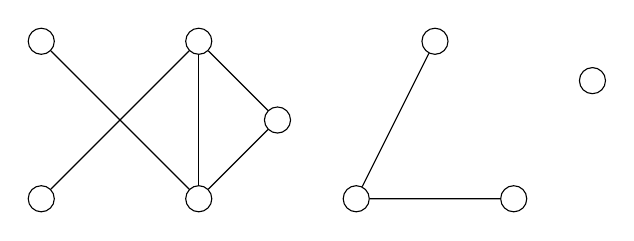
\begin{tikzpicture}
        \node [node] (1) at (0,2) {};
        \node [node] (2) at (2,2) {};
        \node [node] (3) at (0,0) {};
        \node [node] (4) at (2,0) {};
        \node [node] (5) at (3,1) {};

        \node [node] (6) at (5,2) {};
        \node [node] (7) at (4,0) {};
        \node [node] (8) at (6,0) {};

        \node [node] (9) at (7,1.5) {};

        \draw (1) -- (4) -- (5) -- (2) -- (3);
        \draw (2) -- (4);

        \draw (6) -- (7) -- (8);
    \end{tikzpicture}
\end{center}
In this course, we make the following assumptions:
\begin{itemize}
    \item The number of vertices is finite.
    \item No `multiple edges': every pair of vertices is connected by at most one edge.
    \item No loops: no vertex can be joined to itself - edges have to go between different vertices.
\end{itemize}

\subsection{Where do such structures arise?}
% TODO Konigsberg picture

\begin{eg}
    \leavevmode
    \begin{enumerate}[label=\arabic*.]
        \item Problem: Can we walk across each bridge in this city precisely once, returning to our starting point? (Euler, 1736)

            We turn the problem into a graph problem - in particular, a multigraph to allow multiple edges between vertices.  The vertices of this graph are the four bits of the city, while the edges are the seven bridges.
            In terms of this graph, the problem becomes to walk around the edges of this graph precisely once, and return to the starting vertex.

        \item Map colouring problem (1850s)

            How many colours are required to colour a map such that neighbouring countries get different colours?
            (picture)
            Here, the vertices are countries, and the edges are neighbouring pairs.  If we can draw a graph with no crossing edges, how many colours are needed to colour vertices with all edges having two different colours?

        \item Cosets of finite subgroups of finite groups

            Let $G$ be a finite group, $H \leq G$, $|G : H| = n$.  By Lagrange, $\exists a_1, \dots, a_n \in G$ such that the left cosets of $H$ are $a_1 H, \dots a_n H$.
            Similarly, $\exists b_1, \dots, b_n \in G$ such that the right cosets of $H$ are $H a_1, \dots, H a_n$.
            Can we do this simultaneously? In particular, are there $a_1, \dots, a_n \in G$ such that $a_1 H, \dots, a_n H \in G$ are the left cosets, and $H a_1, \dots, H a_n \in G$ are the right cosets?

            In the case where $H \lhd G$ this is easy since we have $a H = H a \; \forall a \in G$.  However it is less obvious if $H \centernot\lhd G$.
            Let $L$ be the set of left cosets, and let $R$ be the set of right cosets. We can create a graph where the vertices are $L \cup R$.
            Join $X \in L$ to $Y \in R$ by an edge if we can find some $a$ such that $X = aH$ and $Y = Ha$, that is, if $X$ and $Y$ have a common element.  Ideally, we would like a graph like this
            (insert bipartite graph here)

            Formally, we ask: In this graph, can we find a set of edges meeting each vertex precisely once?

        \item Fermat equation mod $p$

            Consider the equation $x^n + y^n = z^n$. Does this have solutions mod $p$ for $p$ a prime?  Rule out trivial solutions such as $x = 0, y = z$, in particular we search for solutions in $\mathbb{Z}_p$ where $xyz \ne 0$.
            Let $G = \mathbb{Z} \setminus \{0\}$ under multiplication, and $H = \{g^n : g \in G\}$.  We can check that $H \leq G$, and that $|G : H| \leq n$, by considering the number of $n$th roots an element can have.
            So, $G$ can be partitioned into $g_1 H, g_2 H, \dots, g_mH$ for some $g_1, g_2, \dots, g_m$ and $m \leq n$.  Suppose in some $g_i H$, we have $a, b, c$ with $a + b = c$.  Then $a = g_i x^n, b = g_i y^n, c = g_i z^n$ for some $x, y, z \in G$.  Then
            \begin{align*}
              g_i x^n + g_i y^n &= g_i z^n \\
              x^n + y^n &= z^n
            \end{align*}

            It finally remains to show Schur's Theorem:

            \begin{thm}[Schur's Theorem]\hypertarget{thm:schur}
                Let $n$ be a positive integer. Then if $p$ is a sufficiently large positive integer, whenever $\{1, 2, \dots, p\}$ is partitioned into $n$ parts, we can solve $a + b = c$ with $a, b, c$ all in some part.
            \end{thm}
    \end{enumerate}
\end{eg}

\clearpage
\section{Ramsey Theory}

\begin{defi}[Graph]\hypertarget{def:graph}
    A \textbf{graph} is an ordered pair $(V, E) = G$ where $V$ is a finite set and $E$ is a set of unordered pairs of distinct elements of $V$.
    We call elements of $V$ \textbf{vertices} of $G$ and elements of $E$ \textbf{edges}.
    We often write $v \in G$ to mean $v \in V$ and sometimes, where clear, $e \in G$ to mean $e \in E$.
    Often denote $\{u, v\} \in E$ by $uv$. Note $uv = vu$.
\end{defi}

\begin{eg}
    Here's an example of a \hyperlink{def:graph}{graph} $G = (\{1, 2, 3, 4, 5, 6, 7\}, \{12, 23, 13, 14, 67\})$, but it's often easier to represent a graph by a drawing: take a point for each \hyperlink{def:graph}{vertex}, join two vertices if they are in an \hyperlink{def:graph}{edge}.
    \begin{center}
        \begin{tikzpicture}[every node/.style = node]
            \node [label=left:$1$]  (1) at ( -1,  0)  {};
            \node [label=above:$2$] (2) at (  0,  1)  {};
            \node [label=below:$3$] (3) at (  0, -1)  {};
            \node [label=right:$4$] (4) at (  1,  0)  {};

            \node [label=above:$5$] (5) at (2.5,  0)  {};
            \node [label=above:$6$] (6) at (  4,  0)  {};
            \node [label=above:$7$] (7) at (5.5,  0)  {};

            \draw (4) -- (1) -- (2) -- (3) -- (1);
            \draw (6) -- (7);
        \end{tikzpicture}
    \end{center}
\end{eg}

\begin{defi}[Isomorphism]\hypertarget{def:gIso}
    Let $G = (V, E)$ and $G' = (V', E')$ be \hyperlink{def:graph}{graphs}.
    An \textbf{isomorphism} from $G$ to $G'$ is a bijection $\phi: V \to V'$ such that for all $u, v \in V$, we have $\phi(u) \phi(v) \in E'$ if and only if $u v \in E$.
    If such an isomorphism exists, we say $G$ is \textbf{isomorphic} to $G'$.
\end{defi}

\begin{defi}[Subgraph]\hypertarget{def:subgraph}
    Suppose also $H = (W, F)$ is a \hyperlink{def:graph}{graph}.
    We say $H$ is a \textbf{subgraph} of $G$ and write $H \subset G$ if $W \subset V$ and $F \subset E$.
    Often, we say `$H$ is a subgraph of $G$' to mean `$H$ is \hyperlink{def:gIso}{isomorphic} to a subgraph of $G$'.
\end{defi}

\begin{defi}[Complete graph of order $n$]\hypertarget{def:Kn}
    The \textbf{complete graph of order $n$}, $K_n$ has $n$ vertices with every pair forming an edge.
\end{defi}

\begin{center}
    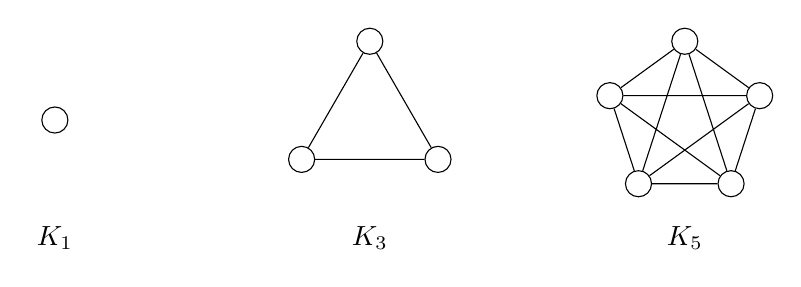
\begin{tikzpicture}
        \begin{scope}
            \node [node] (A) at (0, 0) {};
            \node at (0, -1.5) {$K_1$};
        \end{scope}

        \begin{scope}[xshift=4cm]
            \node [node] (A) at (  90:1)  {};
            \node [node] (B) at (-150:1)  {};
            \node [node] (C) at ( -30:1)  {};

            \draw (A) -- (B) -- (C) -- (A);
            \node at (0, -1.5) {$K_3$};
        \end{scope}

        \begin{scope}[xshift=8cm]
            \node [node] (A) at (  90:1)  {};
            \node [node] (B) at ( 162:1)  {};
            \node [node] (C) at (-126:1)  {};
            \node [node] (D) at ( -54:1)  {};
            \node [node] (E) at (  18:1)  {};

            \draw (A) -- (B) -- (C) -- (D) -- (E) -- (A);
            \draw (A) -- (C) -- (E) -- (B) -- (D) -- (A);
            \node at (0, -1.5) {$K_5$};
        \end{scope}
    \end{tikzpicture}
\end{center}

Looking at the diagram, we see $K_3$ looks like a triangle, and we will often just refer to $K_3$ as a \textbf{triangle}\label{def:triangle}.  In addition, note that if $m \leq n$, then $K_m \subset K_n$.

Recall \hyperlink{thm:schur}{Schur's Theorem}:
\begin{thm}[Schur's Theorem reformulated\label{thm:schur2}]
    Let $k$ be a positive integer. Then there is a positive integer $n$ such that if the set $[n] = \{1, 2, \dots, n\}$ is coloured with $k$ colours, we can find $a, b, c$ with $a + b = c$ and $a,b,c$ the same colour.
\end{thm}

Can we prove this directly? First try $k=1$, where $n=2$ immediately works because $1+1=2$.

\newcommand{\red}[1]{\textcolor{bred}{#1}}
\newcommand{\green}[1]{\textcolor{bgreen}{#1}}
\newcommand{\blue}[1]{\textcolor{bblue}{#1}}
\newcommand{\yellow}[1]{\textcolor{byellow}{#1}}

For $k=2$, use colours \red{red} and \green{green}, wlog we can take \red{$1$ red}.
As $\red{1}+\red{1}=2$, we must have a \green{green $2$}.
Similarly, \red{$4$} must be \red{red} otherwise $\green{2}+\green{2}=\green{4}$.
Next, we have $\red{1} + 3 = \red{4}$, so \green{$3$} must be \green{green}.
Finally, notice that $\red{1} + \red{4} = \green{2} + \green{3}$ so $n = 5$ suffices.

This case analysis worked for $k=2$, but is likely to get a lot more fiddly for larger $k$.
Even for $k=3$ this case analysis turns out to be a lot harder, so can we come up with a `better' proof for the $k=2$ case, that is `more likely to generalise'?

\begin{proof}($k=2$ of Schur's Theorem, improved)
    Suppose $[5] = \{1, 2, 3, 4, 5\}$ are coloured \red{red} and \green{green}.
    Then some three of these are the same colour, and without loss of generality $\red{i} < \red{j} < \red{k}$ are \red{red}.
    If $j-i$ is \red{red} we are done, since $\red{i} + \red{(j-i)} = \red{j}$.
    Similarly if $k-i$ or $k-j$ is \red{red}, we are done.
    If not, all of $j-i$, $k-i$, $k-j$ are \green{green}, but then $\green{k-i} = \green{(j-i)} + \green{(k-j)}$, and we are done.
\end{proof}

Let's try a similar approach for $k=3$, and I claim $n=16$ works.

\begin{proof}(Schur's theorem, $k=3$)
    Suppose $[16]$ are coloured \red{red}, \green{green} and \blue{blue}.
    By the pigeonhole principle, some six numbers are the same colour, without loss of generality $\red{x_1} < \red{x_2} < \dots < \red{x_6}$ are \red{red}.
    If $x_j - x_i$ is \red{red} for any $i<j$ then we are done: $\red{x_i} + \red{(x_j - x_i)} = \red{x_j}$.
    So assume all $x_j - x_i$ are \blue{blue} or \green{green}.
    Consider the five numbers $x_2 - x_1$, $x_3 - x_1$, $x_4 - x_1$, $x_5 - x_1$, $x_6 - x_1$.
    By the pigeonhole principle, some three of these are the same colour: say $\green{x_i - x_1}$, $\green{x_j - x_1}$, $\green{x_k - x_1}$ are green, for $i < j < k$.

    If $x_j - x_i$ is \green{green}, we are done: $\green{(x_i - x_1)} + \green{(x_j - x_i)} = \green{x_j - x_1}$, similarly if $x_k - x_i$ or $x_k - x_j$ is \green{green}.
    Otherwise, all of $\blue{x_j - x_i}$, $\blue{x_k - x_i}$, $\blue{x_k - x_j}$ are \blue{blue}, and we have $\blue{(x_j - x_i)} + \blue{(x_k - x_j)} = \blue{x_k - x_i}$, so we are done.
\end{proof}

This last paragraph looks very similar to the proof of the $k=2$ case, so can we use induction? It's unclear, because it wasn't exactly the previous case.  But notice how we always seem to be interested in differences of two numbers, yet we never seem to use facts like $7-3 = 9-5$.
So, consider a graph where the vertices are numbers, and the edges refer to the difference between two vertices, and we colour edges.

Suppose the edges of a \hyperlink{def:Kn}{complete graph} $K_6$ are coloured blue and yellow. Then we can find a monochromatic \hyperref[def:triangle]{triangle}.
\begin{proof}
    Pick $v \in K_6$. $v$ is in five edges, so some three are the same colour, without loss of generality call them $vx, vy, vz$ and say they are \red{red}.
    If any of $xy, xz, yz$ is \red{red}, we have a \red{red triangle} with $v$.
    If not, $xyz$ is a \green{green triangle}.
    \begin{center}
        \begin{tikzpicture}[scale=1.5, every node/.style=node]
            \begin{scope}
                \node[label=left:$v$]   (v) at ( -0.5, 0) {};
                \node[label=above:$x$]  (x) at (60: 1)    {};
                \node[label=right:$y$]  (y) at ( 1, 0)    {};
                \node[label=below:$z$]   (z) at (-60:1)   {};

                \draw[bgreen, very thick] (x) -- (y) -- (z) -- (x);
                \begin{scope}[bred]
                    \draw (v) -- (x);
                    \draw (v) -- (y);
                    \draw (v) -- (z);
                \end{scope}
            \end{scope}
            \begin{scope}[xshift=-3cm]
                \node[label=left:$v$]   (v) at ( -0.5, 0) {};
                \node[label=above:$x$]  (x) at (60: 1)    {};
                \node[label=right:$y$]  (y) at ( 1, 0)    {};
                \node[label=below:$z$]   (z) at (-60:1)   {};

                \draw[bgreen] (y) -- (z) -- (x);
                \begin{scope}[bred]
                    \draw (v) -- (z);
                    \draw[very thick] (x) -- (y) -- (v) -- (x);
                \end{scope}
            \end{scope}
        \end{tikzpicture}
    \end{center}
\end{proof}

\begin{remark}
    Schur for $k=2$ now follows: Suppose $[5]$ are coloured \red{red}/\green{green}. Take a $K_6$ with vertices $\{0, 1, \dots, 5\}$. Colour edge $ij$, $(i<j)$ with the colour of $j-i$.
    By the above proof, we have a monochromatic triangle $abc$ ($a<b<c$). Then $(c-b) + (b-a) = c-a$, and $c-b, b-a, c-a$ are all the same colour.
    We cannot necessarily find a monochromatic triangle in $K_5$, so 6 vertices are necessary.

    \begin{center}
        \begin{tikzpicture}[scale=2, every node/.style=node]
            \node (A) at (  90:1)  {};
            \node (B) at ( 162:1)  {};
            \node (C) at (-126:1)  {};
            \node (D) at ( -54:1)  {};
            \node (E) at (  18:1)  {};

            \draw[bred] (A) -- (B) -- (C) -- (D) -- (E) -- (A);
            \draw[bgreen] (A) -- (C) -- (E) -- (B) -- (D) -- (A);
        \end{tikzpicture}
    \end{center}

    In this graph form, the statement for more colours is now amenable to an induction proof.
\end{remark}

% prop 1
\begin{nprop}
    Let $k$ be a positive integer. Then there is a positive integer $n$ such that whenever the edges of $K_n$ are coloured with $k$ colours we can find a monochromatic triangle.
\end{nprop}

\pgfmathsetseed{1}

\begin{proof}
    Induction on $k$. For $k=1$, $n=3$ works, so consider $k>1$.

    By the induction hypothesis, there exists $m$ such that if $K_m$ is $(k-1)$-coloured, then there is a monochromatic triangle.  Let $n = k(m-1) + 2$.

    Now $k$-colour the edges of $K_n$.  Pick vertex $v$.
    The number of edges containing $v$ is $n-1 = k(m-1)+1$.  So some $m$ of them are the same colour, without loss of generality blue.
    Let $H$ be a $K_m$ joined to $v$ by blue edges. If $H$ contains a blue edge, it makes a blue triangle with $v$.
    If not, $H$ is a $(k-1)$-coloured $K_m$ so by definition of $m$, it contains a monochromatic triangle.
    \begin{center}
        \begin{tikzpicture}[scale=0.5]
            \node [node, label=left:$v$] (v) at (0, 0) {};

            \foreach \theta in {25, 15, ..., -25}
                \draw[bred] (v) -- (\theta+rand*3:6+rand*0.2);

            \begin{scope}[xshift=6.5cm, scale=3]
                \draw plot [smooth cycle, tension=0.8] coordinates {(-180:1) (-120:1.2) (-60:0.8) (0:0.9) (60:1.1) (120:1.3)};
                \node at (0.4, 0.6) {$H$};
            \end{scope}
        \end{tikzpicture}
    \end{center}
\end{proof}

\begin{remark}
    \leavevmode
    \begin{enumerate}
        \item Can think in terms of the following picture (WIP). Eventually, we will run out of colours and get a monochromatic triangle.
            \begin{center}
                \begin{tikzpicture}[scale=0.6, inner sep=0.05cm]
                    \node [node] (a) at ( -7,  0) {};
                    \node [node] (b) at ( -4,  1) {};
                    \node [node] (c) at ( -1, -1) {};
                    \node [node] (d) at (1.7,  0) {};

                    \foreach \theta in {38, 36, ..., -36}{
                        \pgfmathsetmacro\randa{rand}
                        \pgfmathsetmacro\randb{rand}
                        \pgfmathsetmacro\randc{rand}
                        \pgfmathsetmacro\randd{rand}

                        \draw [bred]    (a) -- ++(\theta     + \randb*1.4      : 3   + \randb*0.5);
                        \draw [bgreen]  (b) -- ++(\theta     + \randd*1.3 - 10 : 3   + \randd*0.5);
                        \draw [borange] (c) -- ++(\theta     + \randc*1.2 + 20 : 2.5 + \randc*0.5);
                        \draw [bblue]   (d) -- ++(\theta*0.7 + \randa*1.2 +  5 : 2.3 + \randa*0.5);

                        \draw [bred]    (a) -- (b);
                        \draw [bgreen]  (b) -- (c);
                        \draw [borange] (c) -- (d);
                    }

                    \draw plot [smooth cycle, tension=0.8, xshift=2.0cm, xscale=2.5, scale=3.0] coordinates {(-180:1.0) (-120:1.2) (-60:0.8) (0:0.9) (60:1.1) (120:1.3)};
                    \draw plot [smooth cycle, tension=0.8, xshift=2.8cm, xscale=2.0, scale=2.6] coordinates {(-180:1.0) (-120:1.2) (-60:0.7) (0:0.9) (60:0.9) (120:1.3)};
                    \draw plot [smooth cycle, tension=0.8, xshift=2.9cm, xscale=1.7, scale=1.8] coordinates {(-180:1.0) (-120:1.3) (-60:0.8) (0:0.9) (60:1.1) (120:1.2)};
                    \draw plot [smooth cycle, tension=0.8, xshift=3.9cm, xscale=1.2, scale=1.0] coordinates {(-180:0.9) (-120:0.9) (-60:0.8) (0:1.1) (60:1.4) (120:1.4)};
                \end{tikzpicture}
            \end{center}

        \item How big do we need to take $n$ to be?  Let $f(k)$ be the smallest $n$ that works with $k$ colours. Clearly $f(1) = 3$. Our proof says for $k>1$, $f(k) \leq k \left(f(k-1)-1\right) + 2 \leq k f(k-1)$.  So by induction, $f(k) \leq 3 k!$.
        \item \nameref{thm:schur2} follows immediately in the same way as for the $k=2$ case.
    \end{enumerate}
\end{remark}

Can we find larger monochromatic subgraphs, for instance a monochromatic $K_4$?  Think about two colours at first for simplicity.  Yes, but we need an intermediate step first.

\begin{eg}
    \leavevmode
    \begin{enumerate}
        \item Let $K_{10}$ have edges coloured \red{red}/\green{green}.
            Then there is a \red{red triangle} or a \green{green $K_4$}.
            \begin{proof}
                Take a vertex $v$. It's in $9$ edges so either $v$ is in \red{$4$ red} edges, or in \green{$6$ green} edges.
                \begin{itemize}
                    \item $v$ is in \red{4 red} edges
                        \begin{center}
                            \begin{tikzpicture}[every node/.style=node]
                                \foreach \ver in {0,1} {
                                    \begin{scope}[xshift=\ver*6 cm]
                                        \node [label=left:$v$]  (v\ver) at (-1, 0) {};
                                        \node [label=right:$w$] (w\ver) at ( 90:1) {};
                                        \node [label=right:$x$] (x\ver) at ( 30:1) {};
                                        \node [label=right:$y$] (y\ver) at (-30:1) {};
                                        \node [label=right:$z$] (z\ver) at (-90:1) {};

                                        \begin{scope}[bred]
                                            \draw (x\ver) -- (v\ver) -- (w\ver);
                                            \draw (z\ver) -- (v\ver) -- (y\ver);
                                        \end{scope}

                                        \draw[bgreen] (w\ver) -- (x\ver) -- (y\ver) -- (z\ver) -- (w\ver) -- (y\ver);
                                    \end{scope}
                                }

                                \draw [very thick, bred]   (x0) -- (z0) -- (v0) -- (x0);

                                \draw [very thick, bgreen] (w1) -- (x1) -- (y1) -- (z1) -- (w1) -- (y1);
                                \draw [very thick, bgreen] (x1) -- (z1);
                            \end{tikzpicture}
                        \end{center}

                        If any edge between $w, x, y, z$ is \red{red}, we have a \red{red triangle}.

                        If not, they are all \green{green} and we have a \green{green $K_4$}.

                    \item $v$ is in \green{$6$ green} edges
                        \begin{center}
                            \begin{tikzpicture}[scale=0.6]
                                \node [node, label=left:$v$] (v) at (0, 0) {};

                                \foreach \theta in {25, 15, ..., -25}
                                    \draw [bgreen] (v) -- (\theta+rand*3:5+rand*0.5);

                                \begin{scope}[xshift=5cm, scale=3]
                                    \draw plot [smooth cycle, tension=0.8] coordinates {(-180:1.2) (-120:1) (-60:0.8) (0:0.9) (60:1.1) (120:0.9)};
                                    \node [align=center, rectangle] at (0.4, 0.5) {$H$ \\ $(K_6)$};
                                \end{scope}
                            \end{tikzpicture}
                        \end{center}

                        We know $H$ contains a monochromatic triangle. If it is \red{red}, we are done.  If it is \green{green}, then it makes a \green{green $K_4$} with $v$ as required. \qedhere
                \end{itemize}
            \end{proof}
        \item Let $K_{20}$ be coloured \red{red}/\green{green}. Then $\exists$ a monochromatic $K_4$.
            \begin{proof}
                Pick a vertex $v$. It's in $19$ edges, so some $10$ of them are the same colour, without loss of generality \red{red}.

                Let $H$ be a $K_{10}$ joined to $v$ by \red{red} edges.

                Either $H$ has a \red{red triangle}, making a \red{red $K_4$} with $v$, or $H$ contains a \green{green $K_4$}.
            \end{proof}
    \end{enumerate}
\end{eg}

\begin{defi}[\hypertarget{def:ramseyNum}{Ramsey number}]
    Let $s, t \geq 2$. The Ramsey number $R(s, t)$ is the least $n$ such that whenever $K_n$ has edges coloured \red{red}/\green{green} there must be a \red{red $K_s$} or a \green{green $K_t$} (if such an $n$ exists).
    We also write $R(s) = R(s, s)$.
\end{defi}

We have seen $R(3) = 6$; $R(3, 4) \leq 10$; $R(4) \leq 20$.

\begin{nthm}[Ramsey's Theorem]\label{thm:ramsey}
    $R(s, t)$ exists for all $s, t \geq 2$.  Moreover, if $s, t \geq 2$ then $R(s, t) \leq R(s-1, t) + R(s, t-1)$.
\end{nthm}

\begin{proof}
    Induction on $s+t$.

    For $s=2$, we have $R(2, t) = t$: If all edges of a $K_t$ are \green{green}, then we have a \green{green $K_t$}, otherwise there is a \red{red edge}, which is exactly a \red{$K_2$}.  Similarly $R(s, 2) = s$.

    In the case $s, t > 2$, let $a = R(s-1, t)$ and $b = R(s, t-1)$ which exist by the induction hypothesis.  Let $n = a+b$. Suppose $K_n$ has edges coloured \red{red}/\green{green}.
    Pick $v \in K_n$, which is in $a+b-1$ edges, so either $v$ is in \red{$a$ red edges}, or it is in \green{$b$ green edges}.
    \begin{itemize}
        \item If $v$ is in \red{$a$ red edges}, let $H$ be the $K_a$ joined to $v$ by \red{red} edges.  Now $a = R(s-1, t)$, so either $H$ has a \red{red $K_{s-1}$}, making a \red{red $K_s$} with $v$, or $H$ has a \green{green $K_t$}, so done.
        \item If $v$ is in \green{$b$ green edges}, and we can make the same argument with colours reversed.
    \end{itemize}
\end{proof}

% cor 3
\begin{ncor}
    For all $s, t \geq 2$, $R(s, t) \leq 2^{s+t}$, so $R(s) \leq 4^s$.
\end{ncor}

\begin{proof}
    Induction on $s + t$.  Base cases $s=2$, $R(2, t) = t \leq 2^{2+t}$ and similarly for $t=2$, $R(s, 2) = s \leq 2^{s+2}$.
    For $s, t \geq 2$
    \begin{align*}
        R(s, t) &\leq R(s-1, t) + R(s, t-1) \\
                &\leq 2^{s-1+t} + 2^{s+1-t} \\
                &= 2^{s+t}. \qedhere
    \end{align*}
\end{proof}

\begin{remark}
    \leavevmode
    \begin{itemize}
        \item A more careful version of the same proof gives $R(s) = \mathcal{O} \left(\frac{4^s}{\sqrt{s}}\right)$ (Erd\H{o}s-Szekeres 1935)
        \item A harder proof gives an improvement to $R(s) = \mathcal{O}\left(\frac{4^s}{s}\right)$ (Thomason 1988)
        \item An even harder proof gives $R(s) = \mathcal{O}\left(\frac{4^s}{s^k}\right)$ for any $k$ (Conlon 2009)
        \item Is $R(s) = \mathcal{O}\left((3.999999999)^s\right)$? Unknown.
    \end{itemize}
\end{remark}

\begin{nthm}[Multicolour Ramsey Theorem]\label{thm:multiRamsey}
    Let $k \geq 1$ and $s \geq 2$. Then there exists some $n$ such that whenever the edges of $K_n$ are coloured with $k$ colours, we can find a monochromatic $K_s$.
\end{nthm}

\begin{proof}
    Induction on $k$. For the base case $k=1$, we can take $n=s$.

    For $k>1$, by the induction hypothesis we can find $m$ such that if $K_m$ is $(k-1)$-coloured, then there is a monochromatic $K_s$.
    Let $n = R(s, m)$ and colour $K_n$ with $k$ colours, including \red{red} but not green.
    Re-colour by turning all non-red edges \green{green}.
    By definition of $n$, we have either
    \begin{itemize}
        \item A \red{red $K_s$}, so done
        \item A \green{green $K_m$}. Then in the original colouring, this $K_m$ was $(k-1)$-coloured, so by definition of $m$, it contains a monochromatic $K_s$.
    \end{itemize}
\end{proof}

\begin{remark}
    \leavevmode
    \begin{enumerate} % 1.
        \item We write $R_k(s)$ for the smallest $n$ that works. In particular $R_1(s) = s$ and $R_2(s) = R(s)$.
            Proof of theorem 4 will give $R_k(s) \leq 4^{s^{k-1}}$.
        \item What do we really mean by colouring?
            We have informally talked about `red edges' etc. More formally, we colouring of the edges of $G = (V, E)$ with $k$ colours is a function $c: E \to [k]$. We mostly refer to the colours as `red', `green' and so on.
            We say $H = (W, F)$ is monochromatic if $c |_F$ is constant.
    \end{enumerate}
\end{remark}

With any number of colours, we can find arbitrarily large monochromatic subgraphs. What about infinite ones?

\begin{defi}[Infinite graph]\hypertarget{def:infGraph}
    An \textbf{infinite graph} is an ordered pair $G = (V, E)$ where $V$ is an infinite set and $E$ is a set of unordered pairs of elements of $V$. Note, in our terminology, an infinite graph is not a graph.
\end{defi}

\begin{defi}[(Possibly infinite) graph]\hypertarget{def:dumbDefi}
    A \textbf{(possibly infinite) graph} is a graph or an infinite graph.
\end{defi}

\begin{defi}[Infinite complete graph]\hypertarget{def:kInf}
    $K_\infty$ is the infinite graph with a countably infinite vertex set and every pair of vertices forming an edge.
\end{defi}

Where it makes sense to do so, we carry terminology over from graphs to infinite graphs.
Suppose edges of $K_\infty$ are coloured blue/yellow. What can we find? By \nameref{thm:ramsey}, we can find a monochromatic $K_s$ for every finite $s = 1, 2, 3, \dotsc$. Note this doesn't immediately give a monochromatic $K_\infty$:
% \begin{center}
%     \begin{tikzpicture}[inner sep=0.05cm, every node/.style = node, scale=0.6]
%         \begin{scope}
%             \path [scope fading=east] (18, -3) rectangle (25.5, 3);
%             \node (11) at (3, 0) {};
%             \foreach \n in {2,...,9} {
%                 \begin{scope}[xshift=3*\n cm]
%                     \foreach \m in {1,...,\n}{
%                         \node (\n\m) at (360/\n*\m+90: 1) {};
%                     }
%                     \foreach \x in {1,...,\n}{
%                         \foreach \y in {1,...,\x} {
%                             \draw[bred] (\n\x) -- (\n\y);
%                         }
%                     }
%                 \end{scope}
%             }
%             \begin{scope}[on background layer]
%                 \foreach \a in {3,...,9} {
%                     \pgfmathsetmacro\biggest{\a-1}
%                     \foreach \b in {2,...,\biggest} {
%                         \foreach \c in {1,...,\a} {
%                             \foreach \d in {1,...,\b} {
%                                 \pgfmathsetmacro\adist{cos(360/\a*\c)}
%                                 \pgfmathsetmacro\bdist{cos(360/\b*\d)}
%                                 \pgfmathsetmacro\atop{\adist>0.2?1:0}
%                                 \pgfmathsetmacro\abot{\adist<-0.2?1:0}
%                                 \pgfmathsetmacro\btop{\bdist>0.2?1:0}
%                                 \pgfmathsetmacro\bbot{\bdist<-0.2?1:0}
%                                 \pgfmathsetmacro\top{\atop+\btop==2?1:0}
%                                 \pgfmathsetmacro\bot{\abot+\bbot==2?1:0}
%                                 \ifthenelse{\top=1}{\draw [bgreen, opacity=0.1] (\a\c) to [bend right] (\b\d)}
%                                 {
%                                     \ifthenelse{\bot=1}{\draw [bgreen, opacity=0.1] (\a\c) to [bend left] (\b\d)}
%                                     {\draw [bgreen, opacity=0.05] (\a\c) to (\b\d)};
%                                 };
%                             }
%                         }
%                     }
%                 }
%             \end{scope}
%         \end{scope}
%     \end{tikzpicture}
% \end{center}

In the diagram, we see that for any finite $s$ we have a blue $K_s$ but no blue $K_\infty$.  (However in this example, there is a yellow $K_\infty$)

\begin{nthm}[Infinite Ramsey Theorem]\label{thm:infRamsey}
    Let $k \geq 1$. Whenever the edges of $K_\infty$ are $k$-coloured, we have a monochromatic $K_\infty$ subgraph.
\end{nthm}

\begin{proof}
    Take $v_1 \in K_\infty$.  The vertex $v_1$ is in infinitely many edges, so infinitely many edges from $v_1$ are the same colour.
    Let $A_1$ be an infinite set of vertices of $K_\infty$ such that for all $u \in A_1$, $v_1 u$ has colour $c_1$.
    Now pick $v_2 \in A_1$. SImilarly, we can find an infinite $A_2 \subset A_1$ such taht all edges $v_2 u$ for ($u \in A_2$) have colour $c_2$.
    Keep going. We get infinite seuqences $v_1, v_2, v_3, \dotsc$ of vertices, $c_1, c_2, c_3, \dotsc$ of colours and $A_1 \supset A_2 \supset A_3 \supset \dots$ such that
    \begin{itemize}
        \item for $i \geq 2$, $v_i \in A_{i-1}$
        \item for $i \geq 1$, for all $u \in A_i$, $v_i u$ is an edge of colour $c_i$.
    \end{itemize}
    In particular, if $i < j$ then $v_i v_j$ has colour $c_i$. Now, infinitely many of the $c_i$ are the same.
    Say $i_1 < i_2 < i_3 < \dots$ such that $c_{i_1} = c_{i_2} = c_{i_3} = \dotsc$.
    Consider $v_{i_1}, v_{i_2}, v_{i_3}, \dotsc$. Any edge between two of these vertices has colour $c_{i_1}$. So we have a monochromatic $K_\infty$.
\end{proof}

\begin{remark}
    This is often called a `two-pass proof'. On the first pass, we found a sequence of colours, and on the second pass we found infinitely many colours the same.
\end{remark}

\begin{ncor}
    Any bounded sequence has a convergent subsequence.
\end{ncor}

\begin{proof}
    Any bounded monotone seuqence converges, so it is enough to show that any real sequence $(x_n)_{n \geq 1}$ has a monotone subsequence.
    Let $G$ be a $K_\infty$ with vertex set $\set{1, 2, 3, \dotsc}$. Colour $ij$, with $i<j$ blue if $x_i < x_j$ and yellow if not.

    By infinite Ramsey, there is a monochromatic subgraph $H \cong K_\infty$. Let the vertices of $H$ be $n_1 < n_2 < n_3 < \dots$.
    If $H$ is blue, then $(x_{n_j})_{j \geq 1}$ is decreasing, whereas if $H$ is yellow then $(x_{n_j})_{j \geq 1}$ is increasing.
\end{proof}

\subsection{Basic Terminology}

Let $G = (V, E)$ be a graph. Sometimes write $V(G) = V$, and $E(G) = E$.
The \textbf{order} of $G$ is $\abs{G} = \abs{V(G)}$. We denote the number of edges of $G$ by $e(G) = |E(G)|$, sometimes called the size of $G$.

Note that the \hyperlink{def:Kn}{complete graph of order $n$} has order $n$.

\begin{defi}[Neighbourhood\hypertarget{def:neighbour}]
    Let $v \in G$. Then \textbf{neighbourhood} of $v$ is the set
    \begin{equation*}
        \Gamma(v) = \set{w \in G | vw \in E(G)}
    \end{equation*}

    If $w \in \Gamma(v)$, then $w$ is a \textbf{neighbour} of $v$, or $w$ is \textbf{adjacent} to $v$, we write $w \sim v$.
\end{defi}

\begin{defi}[Degree\hypertarget{def:degree}]
    The \textbf{degree} of $v$ is $d(v) = \abs{\Gamma(v)}$, the number of vertices \hyperlink{def:neighbour}{adjacent} to $v$.

    The \textbf{maximum degree} of $G$ is $\Delta(G) = \max_{v \in G} d(v)$

    The \textbf{minimum degree} of $G$ is $\delta(G) = \min_{v \in G} d(v)$

    The \textbf{average degree} of $G$ is $\frac{1}{\abs{G}} \sum_{v \in G} d(v)$
\end{defi}

Clearly $\delta(G) \leq \text{average degree of } G \leq \Delta(G)$.

\begin{defi}[Regular\hypertarget{def:regular}]
    If every vertex in $G$ has the same degree, we say $G$ is \textbf{regular}.

    If this degree is $r$, say $G$ is \textbf{$r$-regular}.
\end{defi}

\begin{eg}
    How do vertex-degrees relate to $e(G)$?  We can count `ends of edges' in two different ways. In particular, each edge has two ends, so there are $2 e(G)$ ends. A vertex $v$ is in $d(v)$ ends, so there are $\sum_{v \in G} d(v)$ ends, and hence  $\sum_{v \in G} d(v)= 2 e(G)$.

    Hence also the average degree of $G$ is $\frac{2e(G)}{\abs{G}}$.
\end{eg}

\begin{defi}[Path\hypertarget{def:path}]
    Let $G$ be a graph. A \textbf{path} in $G$ is a finite sequence $v_0, v_1, \dotsc, v_l$ of distinct vertices of $G$ with $v_{i-1} \sim v_i$ for $1 \leq i \leq l$.

    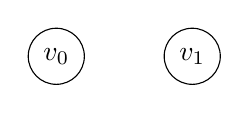
\begin{tikzpicture}
        \node [node] (0) {$v_0$};
        \node [node] [right=of 0] {$v_1$};
    \end{tikzpicture}

    We say this path has length $l$ and goes from $v_0$ to $v_l$.

    If $v, w \in G$ we write $v \to w$ to mean there is a path from $v$ to $w$.
\end{defi}

The relation $\to$ is an equivalence relation (Exercise.) % TODO thing about transitivity

\begin{defi}[Components\hypertarget{def:components}]
    The equivalence classes of $\to$ are called the \textbf{components} of $G$. If $G$ has only one component, we say $G$ is \textbf{connected}.
    % TODO diagram of components
\end{defi}

\begin{defi}[Cycle\hypertarget{def:cycle}]
    A \textbf{cycle} is a sequence $v_0, v_1, \dotsc, v_l$ of vertices of $G$ with $v_0, \dots, v_{l-1}$ distinct, $v_l = v_0$, $v_{i-1} \hypertarget{def:path}{\sim} v_i$ for $1 \leq i \leq l$ and $l \leq 3$.
    We say that the length of the cycle is $l$.
    % TODO cycle diagram
\end{defi}

\begin{defi}[Forest\hypertarget{def:tree}]
    % TODO forest diagram
    A graph with no cycles is called a \textbf{forest}.  A \textbf{tree} is a connected forest. Each component of a forest is a tree.
\end{defi}

\begin{defi}[Disjoint union\hypertarget{def:disUnion}]
    Suppose $G$, $H$ are graphs with $V(G) \cap V(H) = \emptyset$. The \textbf{disjoint union} of $G, H$ is the graph $G \cup H$ with $V(G \cup H) = V(G) \cup V(H)$ and $E(G \cup H) = E(G) \cup E(H)$.

    We often write $G \cup H$ even if $V(G) \cap V(H) \neq \emptyset$, this means take graphs $G', H'$ with $G' \cong G$, $H' \cong H$, $V(G') \cap V(H') = \emptyset$ then take $G' \cup H'$.
\end{defi}

\begin{eg}
    \leavevmode
    \begin{enumerate}
        \item $K_3 \cup K_5$ % TODO diagram here
        \item Any graph is the disjoint union of its components $(G_1 \cup \dots \cup G_k)$.
            For instance, a forest is a \hyperlink{def:disUnion}{disjoint union} of trees.
    \end{enumerate}
\end{eg}

\begin{defi}[Induced subgraph\hypertarget{def:indSubgraph}]
    Let $G = (V, E)$ be a graph, and let $W \subset V$. The \textbf{induced subgraph} on $W$ is the graph $G[W]$ with $V(G[W]) = W$ and, for $x,y \in W$, $xy \in E(G[W]) \iff xy \in G$.
\end{defi}

\begin{defi}[Complement\hypertarget{def:complement}]
    Let $G = (V, E)$ be a graph. The \textbf{complement} of $G$ is the graph $\overline{G}$ with $V(\overline{G}) = V$, and for distinct $x, y \in V$, $xy \in E(\overline{G}) \iff xy \notin E$.
\end{defi}

\begin{eg}
    \leavevmode
    \begin{itemize}
        \item Suppose edges of $K_n$ are coloured blue/yellow. We can think about the `blue subgraph' with $n$ vertices and blue edges only. The complement is the yellow subgraph.
        \item % TODO self complement
    \end{itemize}
\end{eg}

\begin{notation}
    Let $f, g: \N \to (0, \infty)$.
    We say
    \begin{itemize}[label={--}]
        \item $f = \mathcal{O}(g)$ if $f < A g$ for some constant $A$.
        \item $f = \Omega(g)$ if $g = \mathcal{O}(f)$
        \item $f = \Theta(g)$ if $f = \mathcal{O}(g)$ and $f = \Omega(g)$.

        \item $f = o(g)$ means $f/g \to 0$ (as $n \to \infty$)
        \item $f = \omega(g)$ means $f/g \to \infty$
        \item $f \sim g$ means $f/g \to 1$.
    \end{itemize}
\end{notation}

\section{Extremal Graph Theory}

\paragraph{Problem} (from (link) section 1): How large must $n$ be so that if edges of $K_n$ are coloured blue/yellow then always get a monochromatic $K_s$?

Let $G$ be a `blue subgraph' of $K_n$, consisting of all vertices, and only the blue edges.
$K_n$ has a blue $K_s \iff K_s \subset G$, and $K_n$ has a yellow $K_s \iff G$ has an induced $\overline{K_s}$ subgraph.

\paragraph{rephrase}
How large must $n$ be to force every graph of order $n$ to have $K_s$ or $\overline{K_s}$ as an induced subgraph?

This is a typical example of an \textbf{extremal problem}: How large must some parameter of $G$ be to force $G$ to have a certain property?

Alternatively, how big can the parameter be with $G$ not having the property?

\subsection{Forbidden Subgraph Problem}
Fix a graph $H$ with at least one edge. Let $n \geq \abs{H}$. Clearly $H \subset K_n$ but $H \not\subset \overline{K_n}$.

How many edges must a graph $G$ of order $n$ have to force $H \subset G$? Alternatively, if $\abs{G} = n$ and $H \subset G$, how large can $e(G)$ be?

\begin{defi}
    Define
    \begin{equation*}
        \ext(n; H) = \max\set{e(G) | \abs{G} = n, H \not\subset G}
    \end{equation*}
\end{defi}

\paragraph{Problem} Can we determine $\ext(n; H)$?

\subsubsection{Triangles}
Let $H = K_3$. The goal is to find $G$ with $\abs{G} = n$, $e(G)$ large and $\Delta \not\subset G$.

The idea is to partition $V(G) = X \cup Y$ with all edges going from $X$ to $Y$.

\begin{defi}
    A graph $G$ is \textbf{bipartite} (with bipartition $(X, Y)$) if $V(G)$ can be partitioned as $X \cup Y$ in such a way that if $e \in E(G)$ then $e = xy$ for some $x \in X$, $y \in Y$.
\end{defi}

Bipartite graphs have no $\Delta$s (and indeed no cycles of odd length). In fact the converse is also true:
% thm 7
\begin{nthm}\label{thm:7}
    A graph is bipartite iff it contains no odd cycles.
\end{nthm}

\begin{proof}
    May return to this later, an exercise for now.
\end{proof}

Which bipartite graph is best?

Clearly it is a good idea to include all possible edges from $X$ to $Y$.

\begin{defi}
    Let $s, t \geq 1$. The \textbf{complete bipartite graph} $K_{s, t}$ has bipartition (X, Y) with $\abs{X} = s$, $\abs{Y} = t$ and $xy \in E(K_{s, t})$ $\forall x \in X, y \in Y$.
\end{defi}

We have $\abs{K_{s, t}} = s + t$ and $e(K_{s, t}) = st$, and aim to maximise $st$ subject to $s + t = n$, that is, maximise $s(n-s)$.
So, the best bipartite graph is $K_{\ceil{\frac{n}{2}}, \floor{\frac{n}{2}}}$

But what if some non-bipartite graph is better?
In fact, the bipartite graph always wins:

% thm 8
\begin{nthm}[Mantel's Theorem\label{thm:8}]
    Let $n \geq 3$. Suppose $\abs{G} = n$, $e(g) \geq \floor{\frac{n^2}{4}}$ and $\Delta \not\subset G$.
    Then $G \cong K_{\ceil{\frac{n}{2}}, \floor{\frac{n}{2}}}$
\end{nthm}

\begin{proof}
    Induction on $n$. Start with the $n=3$ case:
    \paragraph{$n=3$}: Consider $K_{2, 1}$, it satisfies $\abs{G} = 3$, $e(G) \geq 2$, $\Delta \subset G$, as required.
    \paragraph{$n>3$}: Let $\abs{G} = n$, $e(G) \geq \floor{\frac{n^2}{4}}$, $\Delta \subset G$.

    First, remove edges from $G$ if necessary to get $H$ with $\abs{H} = n$, $e(H) = \floor{\frac{n^2}{4}}$. Clearly $\Delta \not\subset H$.

    Let $v \in H$ with $d(v) = \delta(H)$ and let $K = H - v$ (ie $H$ with vertex $v$ and all edges including $v$ removed). Now, $\abs{K} = n-1$, $\Delta \not\subset K$ and $e(K) = \floor{\frac{n^2}{4}} - \delta(H)$.

    Suppose $n$ is even. Then $\delta(H) \leq \text{average degree of H } = \frac{2 e(H)}{H} = \frac{n^2/2}{n} = \frac{n}{2}$.
    Hence $e(K) \geq \frac{n^2}{4} - \frac{n}{2} = \frac{n^2 - 2n}{4} = \frac{n^2 - 2n + 1}{4} - \frac{1}{4} = \frac{(n-1)^2}{4} - \frac{1}{4} = \floor{\frac{(n-1)^2}{4}}$
    Similarly if $n$ odd, also get $e(K) \geq \floor{\frac{(n-1)^2}{4}}$. Hence by the induction hypothesis, $K \cong K_{\ceil{\frac{n-1}{2}, \floor{\frac{n-1}{2}}}}$.

    Also $d(v) = e(H) - e(K)$.
    If $n$ even, $d(v) = \frac{n^2}{4} - \frac{n^2 - 2n}{4} = \frac{n}{2}$.
    $H$ is formed by adding a vertex $v$ to $K \cong K_{\frac{n}{2}, \frac{n-2}{2}}$ and joining $v$ to $\frac{n}{2}$ vertices of $K$, without creating a $\Delta$.

    If $K$ has bipartition $(X, Y)$, $v$ cannot be joined both to a vertex in $X$ and a vertex in $Y$. So $v$ must be joined to all vertices in the larger of $X$, $Y$.

    Thus $H \cong K_{\ceil{\frac{n}{2}}, \floor{\frac{n}{2}}}$ and similarly if $n$ is odd.

    We recover $G$ by adding edges to $H$ without making a $\Delta$. But any new edge creates a $\Delta$, so $G \cong H$.
\end{proof}

Hence if $\abs{G} = n$, $e(G) > \floor{\frac{n^2}{4}}$ then $\Delta \subset G$. Therefore $\ext(n; \Delta) = \floor{\frac{n^2}{4}}$.

\subsubsection{Complete graphs}
% what about K4? try a tri-partite

% def r-partite
\begin{defi}
    A graph $G$ \textbf{$r$-partite}  if we can partition $V(G) = X_1 \cup \dotsb \cup X_r$ in such a way that if $xy \in E(G)$ then $x \in X_i, y \in X_j$ for some $i \neq j$.
    We say $G$ is \textbf{complete $r$-partite} if whenever $x \in X_i$, $y \in X_j$ with $i \neq j$ then $x y \in E(G)$.
\end{defi}

% def turan graph finish!!
\begin{defi}
    The \textbf{Tur\'{a}n graph} $T_r(n)$ is the complete $r$-partite graph with $n$ vertices and vertex-classes as equal as possible. Write $t_r(n) = e(T_r(n))$.
\end{defi}

\begin{eg}
    \leavevmode
    \begin{itemize}
        \item $T_2(n) = K_{\floor{\frac{n}{2}}, \ceil{\frac{n}{2}}}$
        \item The diagram shows $T_3(7)$.
    \end{itemize}
\end{eg}

Properties of the Tur\'{a}n graph
\begin{enumerate}
    \item $K_{r+1} \not\subset T_r(n)$. If we add an edge to $T_r(n)$ we create a $K_{r+1}$.
    \item $T_r(n)$ has more edges than any other $r$-partite graph on $n$ vertices. Suppose $G$ is a complete $r$-partite graph with some two vertex classes $X, Y$ with $\abs{Y} > \abs{X}+1$.
        Moving a vertex from $Y$ to $X$ loses $\abs{X}$ edges but gains $\abs{Y}-1 > \abs{X}$ edges.
    \item If $r \mid n$ then all classes of $T_r(n)$ are same.
        If $r \nmid n$ then we have `small' classes, with $k$ vertices, say, and `big' classes with $k+1$ vertices.
    \item If $r \mid n$ then $T_r(n)$ is regular.
        If $r \nmid n$ then if $v$ in big class, $d(v) = \delta(T_r(n))$ and if $v$ is in the small class $d(v) = \Delta(T_r(n)) = \delta(T_r(n)) + 1$
        So in general, vertex degrees in $T_r(n)$ differ by at most 1.
    \item Deleting a vertex of minimal degree from $T_r(n)$ removes a vertex from a big class, thus making $T_r$ (n-1).
        So $t_r(n-1) = t_r(n) - \delta(T_r(n))$.
    \item Suppose we have $T_r(n-1)$. Add a vertex $v$. How many edges can we add without creating a $K_{r+1}$? We can't join $v$ to a vertex in every class so must miss some class.
        So the best is to join $v$ to all vertices except those in a particular small class $X$.
        Same as adding $v$ to class $X$, so we've made $T_r(n)$. So \# of edges we can add is at most $t_r(n) - t_r(n-1)$ and only way to achieve this makes $T_r(n)$.
\end{enumerate}

% thm 9
\begin{nthm}[Tur\'{a}n's Theorem\label{thm:9}]
    Let $r \geq 2$ and $\abs{G} = n \geq r+1$. If $e(G) \geq t_r(n)$ and $K_{r+1} \not\subset G$ then $G \cong T_r(n)$.
\end{nthm}

\begin{proof}
    Induction on $n$.
    $n = r+1$. $T_r(r+1)$ has one class of 2 vertices, rest with 1 vertex each. So $T_r(r+1)$ is $K_{r+1}$ with 1 edge removed. So $G \cong T_r(r+1)$.
    % diagram

    $n > r+1$. First delete edges from $G$ to form subgraph $H$ with $\abs{H} = n$, $e(H) = t_r(n)$ and $K_{r+1} \not \subset H$. Let $v \in H$ have minimal degree and let $K = H- v$.
    We know $\abs{H} = \abs{T_r(n)}$ and $e(H) = e(T_r(n))$ so $H$ and $T_r(n)$ have same average degree. But degrees in $T_r(n)$ are as equal as possible by (4).

    So $\delta(H) \leq \delta(T_r(n))$. Thus $\abs{K} = n-1$, $K_{r+1} \not\subset K$ and $e(K) = e(H) - \delta (H) \geq e(H) - \delta(T_r(n)) = t_r(n) - \delta(T_r(n)) = t_r(n-1)$ by 5.

    So by induction hypothesis, $K \cong T_r(n-1)$. And $d(v) = e(H) - e(K) = t_r(n) - t_r(n-1)$.
    To recover $H$, we must add a vertex and $t_r(n) - t_r(n-1)$ edges to $K$ without creating a $K_{r+1}$. So by 6, $H \cong T_r(n)$.
    To recover $G$, add edges to $H$ without creating a $K_{r+1}$. But by (1) we can't add any edges. So, $G \cong T_r(n)$.
\end{proof}

So if $r \geq 2$, $n \geq r+1$, $\ext(n, K_{r+1}) = t_r(n)$.

How big is $t_r(n)$ approximately?
Each vertex is joined to a proportion approximately $1 - \frac{1}{r}$ of all vertices, so we have a proportion approx $1 - \frac{1}{r}$ of all possible edges. So $\ext(n; K_{r+1}) \approx (1-\frac{1}{r}) \binom{n}{2}$.
More precisely,

% cor 10
\begin{ncor}\label{cor:10}
    Let $r \geq 2$. As $n \to \infty$, $\ext(n; K_{r+1}) \sim (1 - \frac{1}{r}) \binom{r}{2}$
\end{ncor}

% 2.1.3
\subsubsection{Bipartite graphs}
Can think of cycles and paths as graphs (ignore direction and start point). The graph $C_n$ is cycle of length $n$ eg $C_5$.

\begin{defi}
    The \textbf{cyclic graph of order $n$}, is the cycle of length $n$, called $C_n$.
    % draw C_5
\end{defi}

\begin{defi}
    The \textbf{path graph} of order $n$ is the path of length $n$, called $P_n$.
    % draw P_3
\end{defi}

So $\abs{C_n = n}$, $\abs{P_n} = n+1$, and $e(C_n) = e(P_n) = n$.

\begin{eg}
    What can we say about $\ext(n; C_4)$? Note $C_4 \cong K_{2, 2}$.
    % TODO draw K2 2
    $C_4$ is made from two copies of $P_2$. Suppose $G$ is a graph, $\abs{G} = n$, $e(G) = m$, and $C_4 \not\subset G$. How many $P_2$ subgraphs does $G$ have?
    % TODO draw C_4 as two copies of P_2$

    Given $v \in G$, $v$ is the middle vertex of $\binom{d(v)}{2}$ $P_2$s.
    So the total number of $P_2$s is $\sum_{v \in G} \binom{d(v)}{2}$.

    Instead, observe that if $\{x, y\} \subset V(G)$ with $x \neq y$ then there is at most one $P_2$ where $x, y$ are end vertices (because $C_4 \not\subset G$). So, the number of $P_2$s is $\leq \binom{n}{2}$.
    % TODO draw v as the middle vertex of a <$

    Hence \begin{equation*}\sum_{v \in G} \binom{d(v)}{2} \leq \binom{n}{2}\end{equation*}

    Recall Jensen's Inequality: for a convex function $f$,
    \begin{equation*}
        \frac{1}{n} \sum_{i=1}^n f(x_i) \geq f\left(\frac{1}{n} \sum_{i=1}^n x_i\right)
    \end{equation*}

    Apply Jensen to the earlier bound to give
    \begin{equation*}
        \binom{n}{2} \geq \sum_{v \in G} \binom{d(v)}{2} \geq n \binom{\frac{1}{n} \sum_{v \in G} d(v)}{2} = n \binom{2 \frac{m}{n}}{2}
    \end{equation*}
    Hence $n(n-1) \geq n \frac{2m}{n} (\frac{2m}{n} - 1)$, so $n^2 (n-1) \geq 2m (2m-n)$ so $4m^2 - 2mn - n^2 (n-1) \leq 0$.

    This is a quadratic in $m$ with roots
    \begin{align*}
        m &= \frac{2n \pm \sqrt{4 n^2 + 16 n^2(n-1)}}{8} \\
        &= \frac{n}{4}(1 \pm \sqrt{1 + 4\left(n-1\right)}) \\
        &= \frac{n}{4}\left(1 \pm \sqrt{4n - 3}\right)
    \end{align*}
    Hence $m \leq \frac{n}{4}\left(1 + \sqrt{4n-3}\right)$, so $\ext(n; C_4) \leq \frac{n}{4} \left(1 + \sqrt{4n-3}\right)$, and so $\ext(n; C_4) = \mathcal{O}\left(n^\frac{3}{2}\right)$.

    A similar approach turns out to give a bound on $\ext(n; K_{t, t})$ in general:
    \begin{center}
        \begin{tikzpicture}[every node/.style=node]
            \begin{scope}
                \node (11) at (1,1) {};
                \node (12) at (1,2) {};
                \node (21) at (2,1) {};
                \node (22) at (2,2) {};

                \draw[bred]   (21) -- (11) -- (22);
                \draw[bgreen] (21) -- (12) -- (22);
            \end{scope}

            \begin{scope}[xshift=3cm]
                \foreach \y in {1,2,3} {
                    \node (1\y) at (1, \y) {};
                    \node (2\y) at (2, \y) {};
                };
                \foreach \y in {1,2,3} {
                    \draw[bgreen] (2\y) -- (11);
                    \draw[bred]   (2\y) -- (12);
                    \draw[bblue]  (2\y) -- (13);
                };

            \end{scope}
        \end{tikzpicture}
    \end{center}
\end{eg}

\begin{defi}
    A \textbf{t-fan} in a graph $G$ is an ordered pair $(v, W)$ where $v \in V(G)$, $W \subset V(G)$, $\abs{W} = t$ and $\forall w \in W$, $v \sim w$.
\end{defi}

\begin{eg}
    $2$-fans correspond to $P_2$ subgraphs.
\end{eg}

\begin{nthm}\label{thm:11}
    Let $t \geq 2$. Then $\ext(n; K_{t,t}) = \mathcal{O}\left(n^{2 - \frac{1}{t}}\right)$.
\end{nthm}

\begin{proof}
    Let $\abs{G} = n$, $e(G) = m = \ext(n; K_{t, t})$ and $K_{t,t} \not\subset G$. How many $t$-fans are there in $G$? Each $v \in G$ is in $\binom{d(v)}{t}$ $t$-fans. This total number is $\sum_{v \in G} \binom{d(v)}{t}$.
    Given $W \subset V(G)$ with $\abs{W} = t$, $W$ is in at most $t-1$ $t$-fans (as $K_{t, t} \not\subset G$).

    So the total number of $t$-fans is $\leq \binom{n}{t} (t-1)$.

    Hence
    \begin{align*}
        \binom{n}{t} (t-1) &\geq \sum_{v \in G} \binom{d(v)}{t} \\
                           &\geq n \binom{\frac{1}{n} \sum_{v \in G} d(v)} \qquad \text{by Jensen}\\
                           &= n \binom{\frac{2m}{n}}{t}
    \end{align*}

    So $\frac{n^t}{t!} (t-1) \geq \frac{n}{t!} (\frac{2m}{n} - t)^t$ so $n^t (t-1) \geq n (\frac{2m}{n} - t)^t$.

    If $n$ is sufficiently large (as we may assume) then $m \geq n t$ and so $\frac{m}{n} \geq t$ and so $\frac{2m}{n} - t \geq \frac{m}{n}$.
    Thus $n^t (t-1) \geq n (\frac{m}{n})^t$ so $m^t \leq n^{2t-1} (t-1)$ so $m \leq (t-1)^\frac{1}{t} n^{2-\frac{1}{t}} = \mathcal{O}(n^{2-\frac{1}{t}})$.
\end{proof}

We will see lower bounds later.

Closely related is the \textbf{Problem of Zarankiewicz}. Let $z(n, t)$ be the largest possible number of edges in a bipartite graph $G$ with $n$ vertices in each class and $K_{t, t} \not\subset G$.

\begin{nthm}\label{thm:12}
    Let $t \geq 2$. Then $z(n, t)  = \mathcal{O}(n^{2 - \frac{1}{t}})$.
\end{nthm}
\begin{proof}
    Let $G$ be bipartite with classes $X$, $Y$ with $\abs{X} = \abs{Y} = n$, $e(G) = m = z(n, t)$ and $K_{t, t} \not\subset G$.

    Count number of $t$-fans with vertex in $X$ and set in $Y$.
    Similar to the proof of \cref{thm:11},
    \begin{equation*}
        \binom{n}{t} (t-1) \geq \sum_{v \in X} \binom{d(v)}{t}
    \end{equation*}

    Now $\sum_{v \in X} d(v) = m$, so a similar calculation to \cref{thm:11} gives $m = \mathcal{O}(n^{2 - \frac{1}{t}})$.
\end{proof}

% 2.1.4
\subsubsection{General graphs}

What is $\ext(n; H)$? This is a hard question, and we could not even find an exact answer for $H = C_4$, so instead consider some asymptotics.
Usually $\ext(n; H) \to \infty$ as $n \to \infty$.

Instead what about $\lim_{n \to \infty} \frac{\ext(n; H)}{\binom{n}{2}}$? Does it even exist?

\begin{nprop}\label{prop:13}
    Let $H$ be a graph with at least one edge, and for $n \geq \abs{H}$, let $x_n = \frac{\ext(n; H)}{\binom{n}{2}}$. Then $(x_n)$ converges.
\end{nprop}

\begin{proof}
    Let $n > \abs{H}$, let $\abs{G} = n$, $e(G) = \ext(n; H) = x_n \binom{n}{2}$ and $H \not\subset G$.
    For any $v \in G$, $\abs{G - v} = n-1$ and $H \not\subset G - v$, so $e(G-v) \leq \ext(n-1; H) \ x_{n-1} \binom{n-1}{2}$.
    Each edge $xy \in E(G)$ in $G-v$ for all $v \neq x, y$.
    Hence $(n-2) x_n \binom{n}{2} = (n-2) e(G) = \sum_{v \in G} e(G-v) \leq n x_{n-1} \binom{n-1}{2}$.
    So $x_n \leq x_{n-1}$, so $(x_n)$ is decreasing and bounded below by zero.
\end{proof}

% new lecture

Write $\ext(H) = \lim_{n \to \infty} \frac{\ext(n; H)}{\binom{n}{2}}$ which exists by \cref{prop:13}.
We have seen $\ext(K_{r+1}) = 1 - \frac{1}{r}$, by \cref{cor:10}.
From \cref{thm:11}, $\ext(n, K_{t, t}) = \mathcal{O}(n^{2 - \frac{1}{t}}) = o(n^2) = o(\binom{n}{2})$, so $\ext(K_{t, t}) = 0$.

\begin{fact}
    Tur\'an says that a proportion $1 - \frac{1}{r}$ of edges is enough to guarantee a $K_{r+1}$.
    Increasing this proportion by a tiny amount gives \emph{much} more.
    % draw example
\end{fact}

\begin{defi}
    Write $K_r(t)$ for the complete $r$-partite graph with $t$ vertices in each class (so $K_r(t) = T_r(rt)$).
\end{defi}

\begin{nthm}[Erd\H{o}s-Stone Theorem]\label{thm:14}
    Let $r, t \geq 1$ be integers, and let $\epsilon > 0$ be real.
    Then $\exists n_0$ such that $\forall n \geq n_0$, $\abs{G} = n$, $e(G) \geq (1 - \frac{1}{r} + \epsilon) \binom{n}{2} \implies K_{r+1}(t) \subset G$.
\end{nthm}

\begin{proof}
    % TODO
    Coming soon.
\end{proof}

This is enough to determine $\ext(H)$ for all $H$.

\begin{defi}[Chromatic number]\hypertarget{def:chromNum}
    If $H$ is a graph, the \textbf{chromatic number} of $H$, denoted $\chi(H)$, is the least $r$ such that $H$ is $r$-partite.
\end{defi}

\begin{eg}
    $\Psi(K_r(t)) = r$.
\end{eg}

\begin{ncor}\label{cor:15}
    Let $H$ be a graph with at least one edge. Then
    \begin{equation*}
        \ext(H) = 1 - \frac{1}{\chi(H) - 1}.
    \end{equation*}
\end{ncor}

\begin{proof}
    Let $r = \chi(H) - 1$.
    Then $H$ is $(r+1)$-partite so we can find $t$ such that $H \subset K_{r+1}(t)$ (for instance $t = \abs{H}$ suffices).
    Let $\epsilon > 0$, and take $n_0$ as in \cref{thm:14}.
    Then for all $n \geq n_0$,
    \begin{align*}
        \abs{G} = n, \ e(G) \geq (1 - \frac{1}{r} + \epsilon) \binom{n}{2} &\implies K_{r+1}(t) \subset G \\
                                                                           &\implies H \subset G.
    \end{align*}
    So, for all $n \geq n_0$, $\ext(n; H) < (1 + \frac{1}{r} + \epsilon) \binom{n}{2}$. Hence
    \begin{equation*}
        \ext(H) = \lim_{n \to \infty} \frac{\ext(n; H)}{\binom{n}{2}} \leq 1 - \frac{1}{r} + \epsilon.
    \end{equation*}
    But $\epsilon>0$ was arbitrary, so $\ext(H) \leq 1 - \frac{1}{r}$.

    On the other hand, for all $n$, $H \not\subset T_r(n)$ as $H$ is not $r$-partite. So $\ext(n, H) \geq t_r(n)$, and
    \begin{align*}
        \frac{t_r(n)}{\binom{n}{2}} \to 1 - \frac{1}{r} \quad \text{so} \quad \ext(H) \geq 1 - \frac{1}{r}.
    \end{align*}
\end{proof}

So if $H$ not bipartite, $\ext(H) = 1 - \frac{1}{\chi(H) - 1} \neq 0$, and $\ext(n; H) \sim (1 - \frac{1}{\chi(H) - 1}) \binom{n}{2}$.
This essentially solves the forbidden subgraph problem for non-bipartite $H$.
What about for $H$ bipartite?
\Cref{cor:15} just says $\ext(H) = 0$, i.e. $\ext(n; H) = o(n^2)$, but doesn't tell us for instance that $\ext(n; H)$ grows like a certain power of $n$.
We do however have upper bounds from \cref{thm:11}: $\ext(n, K_{t, t}) = \mathcal{O}(n^{2 - \frac{1}{t}})$.

Another application:
\begin{defi}[Density]\hypertarget{def:density}
    We can define the \textbf{density} of a graph $G$ to be
    \begin{equation*}
        D(G) = \frac{e(G)}{\binom{\abs{G}}{2}} \in [0, 1]
    \end{equation*}
\end{defi}

\begin{eg}
    \leavevmode
    \begin{itemize}
        \item $D(T_r(n)) \to 1 - \frac{1}{r}$ as $n \to \infty$
        \item If $\alpha > \ext(H)$ then if $\abs{G}$ is sufficiently large and $D(G) = \alpha$, we have $H \subset G$.
    \end{itemize}
\end{eg}

Could we define the \hyperlink{def:density}{density} of an infinite graph?
We cannot take the same definition, as we would get $\frac{\infty}{\infty}$.
Instead try something like the `limit of densities of large finite subgraphs'.

\begin{defi}
    The upper density of an infinite graph $G$ is
    \begin{equation*}
        \ud(G) = \lim_{n \to \infty} \sup\set{D(H) | H \subset G, \abs{H} = n}.
    \end{equation*}
\end{defi}

\begin{remark}
    \leavevmode
    \begin{itemize}
        \item Again $\ud(G) \in [0, 1]$.
        \item If $\alpha < \ud(G)$ then for sufficiently large $n$, $G$ has subgraphs of order $n$ and density $\geq \alpha$.
        \item If $\alpha > \ud(G)$ then for sufficiently large $n$, $G$ has no subgraphs of order $n$ and density $\geq \alpha$.
        \item A priori, it seems like $\ud(G)$ could take any value in $[0, 1]$. But surprisingly:
    \end{itemize}
\end{remark}

\begin{ncor}
    For any infinite graph $G$,
    \begin{equation*}
        \ud(G) \in \{0, 1, \frac{1}{2}, \frac{2}{3}, \frac{3}{4}, \dotsc\}.
    \end{equation*}
\end{ncor}

\begin{proof}
    It is enough to show that for $r = 1, 2, 3, \dotsc$,
    \begin{equation*}
        \ud(G) > 1 - \frac{1}{r} \implies \ud(G) \geq 1 - \frac{1}{r+1}.
    \end{equation*}
    Suppose $\ud(G) > 1 - \frac{1}{r}$.  Pick $\alpha$ such that $\ud(G) > \alpha > 1 - \frac{1}{r}$ and fix $n$.
    For sufficiently large $N$, $G$ has subgraphs of order $N$ and density $\geq \alpha > 1 - \frac{1}{r} = \ext(T_{r+1}(n))$.
    So $T_{r+1}(n) \subset G$, but $D(T_{r+1}(n)) \to 1 - \frac{1}{r+1}$ as $n \to \infty$.
    We can do this for every $n$, hence $\ud(G) \geq 1 - \frac{1}{r+1}$.
\end{proof}

\subsubsection{Proof of Erd\H{o}s-Stone}
\Cref{thm:14} says that if a graph $G$ has enough edges, then $K_{r+1}(t) \subset G$.

This condition on $e(G)$ is equivalent to a condition on the average degree.
However, given $d$ and $\delta > 0$ then it turns out that any large graph of average degree $\geq d$ has a large subgraph of minimum degree $\geq d - \delta$.
If $G$ has average degree $d$ and $\abs{G} = n$ large, we can find $\abs{H} = \Omega(n)$ and $\delta(H) \geq d - \delta$ (not proved here. Delete vertices of minimum degree and it works).
So, we have an equivalent version of Erd\H{o}s-Stone with minimum degree condition:

\begin{manualtheorem}{14a}\label{thm:14a}
    Let $r, t \geq 1$ be integers and $\epsilon > 0$ be real. Then $\exists n_0 \; \forall n \geq n_0$,
    \begin{equation*}
        \abs{G} = n, \quad \delta(G) \geq (1 - \frac{1}{r} + \epsilon) n \implies K_{r+1}(t) \subset G.
    \end{equation*}
\end{manualtheorem}

\begin{proof}
    Induction on $r$. Fix $T$ such that

    Then choose $n_0$ such that for all $n \geq n_0$,
    \begin{equation}
        \abs{G} = n, \quad \delta(G) \geq (1 - \frac{1}{r} + \epsilon) n \implies K_{r+1}(t) \subset G.
    \end{equation}
    How? For $r=1$, $K_1(T) \subset G \iff \abs{G} \geq T$. For $r > 1$, $1 - \frac{1}{r} > 1 - \frac{1}{r-1}$ so it follows by inductive hypothesis.

    Suppose the result is not true.
    Then we can find arbitrarily large $n$ and graphs $G$ with $\abs{G} = n$ and $\delta(G) \geq (1 - \frac{1}{r} + \epsilon) n$, $K_{r+1} \not\subset G$.
    Pick such an $n$, $G$ with $n \geq n_0$ and also

    Then we can find $K_r(T) \subset G$, say with vertex classes $X_1, \dotsc, X_r$.
    Let
    \begin{align*}
        A = \set{(W, v_1, \dotsc, v_r) | \abs{W} = t, W \subset V(G), \forall i v_i \in X_i, \forall i, \forall w \in W, v_i \sim W}
    \end{align*}
    % todo picture

    What can we say about $\abs{A}$?
    First, given $v_1 \in X, \dotsc, v_r \in X_r$, we can check from the minimum degree condition that
    \begin{equation*}
        \abs{\Gamma(v_1) \cap \dotsc \cap \Gamma(v_r)} \geq r \epsilon n
    \end{equation*}
    So there are at least $\binom{r \epsilon n}{t}$ choices for $W$. Hence $\abs{A} \geq T^r \binom{r \epsilon n}{t}$.

    On the other hand, given the set $W$, as $K_{r+1}(t) \not\subset G$, we know that there is some $Y_i$ containing at most $t-1$ vertices joined to all of $W$.
    Hence $\abs{A} \leq \binom{n}{t} (t-1) T^{r-1}$, thus
    \begin{equation*}
        T^r \binom{r \epsilon n}{t} \leq \binom{n}{t} (t-1) T^{r-1}.
    \end{equation*}
    Now,
    \begin{equation*}
        \text{RHS} \leq \frac{n^t}{t!} (t-1) T^{r-1}
    \end{equation*}
    while
    \begin{equation*}
        \text{LHS} \geq T^r \frac{1}{t!} (r \epsilon n - t)^t \geq T^r \frac{1}{t!} (\frac{r \epsilon n}{2})^t.
    \end{equation*}
    Combining, we get
    \begin{equation*}
        T^r (\frac{r \epsilon n}{2})^t \leq n^t (t-1) T^{r-1}
    \end{equation*}
    hence $T \leq (\frac{2}{r \epsilon})^t (t-1)$, a contradiction.
\end{proof}

\subsection{Hamiltonian graphs}
\begin{defi}[Hamiltonian]\hypertarget{def:hamil}
    A \textbf{Hamiltonian cycle} in a graph $G$ is a cycle of length $G$, i.e., going through all vertices of $G$.
    If $G$ has a Hamiltonian cycle, we say $G$ is \textbf{Hamiltonian}.
\end{defi}
If $\abs{G} = n$, how big does $e(G)$ need to be to force $G$ \hyperlink{def:hamil}{Hamiltonian}?
This turns out to be uninteresting, we can have $e(G)$ almost $\binom{n}{2}$ and have no Hamiltonian cycle. % add pic

More interestingly, is there a condition on $\delta(G)$?

\begin{nthm}[Dirac's Theorem]\label{thm:17}
    Let $\abs{G} = n \geq 3$ and $\delta(G) \geq \frac{n}{2}$. Then $G$ is Hamiltonian.
\end{nthm}

\begin{remark}
    \leavevmode
    \begin{enumerate}[label=\arabic*.]
        \item This result is best possible:
            % pictures
        \item Of course there are Hamiltonian graphs of smaller minimum degree:
            % picture
        \item In general, given a graph $G$ it is hard computationally to determine if $G$ has a Hamiltonian cycle.
    \end{enumerate}
\end{remark}

\begin{proof}
    First, observe $G$ is connected. Indeed, if $x \neq y$, $x \nsim y$, then $\abs{\Gamma(x) \cup \Gamma(y)} \leq n-2$, but $\abs{\Gamma(x)} + \abs{\Gamma(y)} \geq \frac{n}{2} + \frac{n}{2} = n$ so $\Gamma(x) \cap \Gamma(y) \neq \emptyset$.
    Let $v_0, v_1, \dotsc, v_n$ be a path of maximal length in $G$, say length $k \leq n-1$.
    By maximality, $\Gamma(v_0) \subset \{v_1, \dotsc, v_n\}$. Similarly, $\Gamma(v_k) \subset \{v_0, \dotsc, v_{k-1}\}$.
    If we have some situation like in the % diagram
    diagram, we get a cycle. To be more precise, if
    \begin{equation*}
        A = \set{i \in [k] | v_0 \sim v_i} \quad \text{and} \quad B = \set{i \in [k] | v_k \sim v_{i-1}}
    \end{equation*}
    then $A \cap B \neq \emptyset \implies$ we have a cycle. But $\abs{A \cup B} \leq k < n$ while $\abs{A} + \abs{B} \geq \frac{n}{2} + \frac{n}{2} = n$.
    Hence $\exists i \in A \cap B$ so we have a cycle $C = v_0 v_1 \dotsc v_{i-1} v_k v_{k-1} \dotsc v_i v_0$ of length $k+1$.

    If $k = n-1$, we have a Hamiltonian cycle as required.

    If $k < n-1$, relabel the cycle $C = u_0 u_1 \dotsc u_k u_0$.
    By connectedness, we have some $u_i \in C$ and $w \notin C$ with $w \sim u_i$.
    Then $w u_i u_{i+1} \dotsc u_k u_0 \dotsc u_{i-1}$ is a path of length $k+1$, contradicting maximality.
\end{proof}

\begin{remark}
    The same proof gives the following:
    Let $n > k \geq 3$ and let $G$ be a connected graph $\abs{G} = n$ with $\delta(G) \geq \frac{k}{2}$. Then $G$ contains a path of length $k$ and a cycle of length at least $\frac{k+2}{2}$.
\end{remark}

The Konigsberg bridge problem (link) seems superficially similar, but in fact much less interesting.
\begin{defi}[Euler circuit]\hypertarget{def:euler}
    A \textbf{circuit} of a graph $G$ is a sequence $v_0 v_1 \dotsc v_n$ of vertices of $G$, not necessarily distinct with $v_0 = v_n$, where is $1 \leq i \leq k$ then $v_{i-1} \sim v_i$ and if $1 \leq i < j \leq k$ then edges $v_{i-1} v_i$ and $v_{j-1} v_j$ are distinct.
    It is an \textbf{Euler circuit} if for every $e \in E(G)$, there is some $i$ with $e = v_{i-1} v_i$.
    If $G$ has an Euler circuit we say $G$ is \textbf{Eulerian}.
\end{defi}
% connectedness thing?

\begin{nprop}\label{thm:18}
    Let $G$ be a connected graph. Then $G$ Eulerian $\iff \forall v \in G$, $d(v)$ is even.
\end{nprop}

\begin{proof}
    $\implies$ is obvious: an \hyperlink{def:euler}{Eulerian circuit} must go in and out of a given vertex the same number of times.

    $\impliedby$: use induction on $e(G)$. For $e(G) = 0$ it is clearly true.

    Consider $e(G) > 0$. Let $v_0 v_1 \dotsc v_k = C$ be a circuit in $G$ of maximal length. If $C$ uses all edges of $G$ then we are done.
    If not, delete all edges used in $C$ from $G$ to form $H$.
    In $H$, every vertex still has even degree. Let $H_1$ be a component of $H$ with at least one edge.

    By induction hypothesis, $H_1$ has an Euler circuit $D$.
    Certainly $C, D$ meet at some vertex $v$.
    Join them at $v$ to produce a longer circuit in $G$, a contradiction.
    (Walk along $C$ until we get to $v$, then walk all round $D$ starting/ending at $v$, then walk along the rest of $C$).
\end{proof}

\clearpage
\section{Graph Colouring}
%TODO missing stuff
\end{document}
